\documentclass[12pt,a4paper]{report}

% --- Encoding & Fonts ---
% XeLaTeX xử lý trực tiếp Unicode tiếng Việt; dùng font có đầy đủ ký tự
% thay vì font Latin Modern T1 vốn thiếu nhiều chữ tiếng Việt.
\usepackage{fontspec}
\defaultfontfeatures{Ligatures=TeX}
\setmainfont{Noto Serif}
\setsansfont{Noto Sans}
\setmonofont{DejaVu Sans Mono}

% --- Language ---
\usepackage[vietnamese]{babel}
\usepackage[autostyle]{csquotes} % yeu cau cua biblatex khi dung babel

% csquotes khong kem quote style cho tieng Viet; khong khai bao nay,
% \enquote (dung cho tieu de trong thu muc IEEE) se roi vao fallback
% style va in dau "?" thay vi dau ngoac kep (xac minh bang repro
% 2026-09-27). Dung ngoac kep cong U+201C/U+201D nhu tieng Anh.
\DeclareQuoteStyle{vietnamese}
  {\textquotedblleft}
  {\textquotedblright}
  {\textquoteleft}
  {\textquoteright}

% Cho phep TeX gia them do co gian khi khong tim duoc diem ngat dong
% (cac tieu de tieng Anh dai trong muc luc tai lieu tham khao).
\emergencystretch=2em

% --- Page Layout ---
\usepackage[top=2.5cm, bottom=2.5cm, left=3cm, right=2cm]{geometry}
\usepackage{setspace}
\onehalfspacing

% --- Math ---
\usepackage{amsmath, amssymb, amsfonts}

% --- Graphics & Tables ---
\usepackage{graphicx}
\usepackage{xcolor}
\usepackage{booktabs}
\usepackage{longtable}
\usepackage{tabularx}
\usepackage{array}
\usepackage{caption}
\usepackage{subcaption}

% --- Sơ đồ và đồ thị minh họa ---
\usepackage{tikz}
\usetikzlibrary{arrows.meta,calc,fit,positioning,shapes.geometric}
\usepackage{pgfplots}
\usepgfplotslibrary{groupplots}
\pgfplotsset{compat=1.18}

\definecolor{semgblue}{RGB}{30,90,140}
\definecolor{semggreen}{RGB}{45,125,85}
\definecolor{semgorange}{RGB}{205,110,35}
\definecolor{semgred}{RGB}{175,55,55}
\definecolor{semglight}{RGB}{235,243,249}
\definecolor{semggreenlight}{RGB}{235,247,239}
\definecolor{semgorangelight}{RGB}{252,243,230}
\newcolumntype{Y}{>{\raggedright\arraybackslash}X}
\newcolumntype{P}[1]{>{\raggedright\arraybackslash}p{#1}}

% --- Code Listings ---
\usepackage{listings}

\lstdefinestyle{firmware}{
    language=C,
    basicstyle=\ttfamily\small,
    keywordstyle=\color{blue}\bfseries,
    commentstyle=\color{gray}\itshape,
    stringstyle=\color{red!70!black},
    numbers=left,
    numberstyle=\tiny\color{gray},
    stepnumber=1,
    breaklines=true,
    frame=single,
    tabsize=4,
    showstringspaces=false,
    morekeywords={uint8_t, uint16_t, uint32_t, int8_t, int16_t, int32_t, size_t, HAL_StatusTypeDef}
}
\lstset{style=firmware}

% --- Hyperlinks & References ---
\usepackage[colorlinks=true, linkcolor=blue, citecolor=blue, urlcolor=blue]{hyperref}
\usepackage{cleveref}

% --- Bibliography ---
\usepackage[backend=biber, style=ieee]{biblatex}
\addbibresource{references.bib}

% --- Title Info ---
\title{\textbf{Báo cáo dự án sEMG Firmware}\\
    \large Hệ thống thu nhận và xử lý tín hiệu điện cơ bề mặt}
\author{Tên tác giả}
\date{\today}

\begin{document}

\maketitle
\thispagestyle{empty}
\newpage

\tableofcontents
\listoffigures
\listoftables
\newpage

% ==================== CÁC CHAPTER ====================
% Phiên bản hiện tại của báo cáo chỉ gồm chương lý thuyết sEMG (quyết định
% phạm vi P0, PROJECT_MEMORY.md 2026-09-27). Bộ đếm chương được đặt trước
% để chương này hiển thị là "Chương 2" theo số thứ tự của báo cáo đầy đủ.
% Lưu ý: siunitx đã bỏ khỏi preamble vì gói chưa cài trong môi trường build;
% chương hiện tại không dùng siunitx.
\setcounter{chapter}{1}
\chapter{Cơ sở lý thuyết về sEMG}
\label{ch:semg-theory}

Điện cơ bề mặt (surface electromyography, sEMG) là phép đo hiệu điện thế
vi sai thu được trên bề mặt da do hoạt động điện của các đơn vị vận động
trong vùng thu nhận tạo ra. Vì tín hiệu đi qua nhiều lớp mô và là tổng của
nhiều nguồn, sEMG không phải là phép đo trực tiếp của lực, chuyển động hay
mỏi chủ quan. Chương này trình bày chuỗi hình thành và xử lý tín hiệu theo
trình tự: lệnh vận động, điện thế hoạt động, dẫn truyền thể tích, phép đo,
đặc trưng và diễn giải có điều kiện.

Hình~\ref{fig:signal-chain} tóm tắt chuỗi suy luận đó. Các hình vẽ sơ đồ và
đồ thị định tính trong chương nhằm làm rõ nguyên lý; chúng không đại diện
cho một phép đo sinh lý cụ thể hay một kết quả thực nghiệm của dự án.

\begin{figure}[htbp]
    \centering
    \begin{tikzpicture}[
    stage/.style={draw=semgblue, rounded corners=2pt, fill=semglight,
        align=center, text width=2.05cm, minimum height=1.05cm,
        inner sep=3pt, font=\small},
    arrow/.style={-{Latex[length=2mm]}, semgblue, line width=0.8pt}
]
\node[stage] (command) {Lệnh vận động\\\scriptsize hệ thần kinh trung ương};
\node[stage, right=4mm of command] (mu) {Nơron vận động\\và đơn vị vận động};
\node[stage, right=4mm of mu] (muap) {SFAP $\rightarrow$ MUAP\\\scriptsize chuỗi MUAP};
\node[stage, right=4mm of muap] (volume) {Dẫn truyền thể tích\\và điện cực};
\node[stage, right=4mm of volume] (measure) {$x(t)$\\\scriptsize tín hiệu vi sai};
\node[stage, right=4mm of measure] (features) {Đặc trưng\\và diễn giải có điều kiện};
\draw[arrow] (command) -- (mu);
\draw[arrow] (mu) -- (muap);
\draw[arrow] (muap) -- (volume);
\draw[arrow] (volume) -- (measure);
\draw[arrow] (measure) -- (features);
\node[below=5mm of volume, align=center, text width=6.2cm, font=\footnotesize,
    text=semgred] {Mỗi mũi tên là một phép biến đổi hoặc phép suy luận;\
    chỉ $x(t)$ là đại lượng điện áp được đo trực tiếp.};
\end{tikzpicture}

    \caption{Chuỗi hình thành và diễn giải tín hiệu sEMG. Chỉ hiệu điện thế
    vi sai trên da là đại lượng được đo trực tiếp; các đại lượng còn lại là
    quá trình sinh lý, phép biến đổi tín hiệu hoặc suy luận có điều kiện.}
    \label{fig:signal-chain}
\end{figure}

% ============================================================
\section{Từ lệnh vận động đến điện thế của cơ}
\label{sec:from-command-to-potential}

\subsection{Cấu trúc cơ xương và đơn vị vận động}
\label{sec:motor-unit}

Cơ xương được tổ chức thành các bó cơ; mỗi bó gồm nhiều sợi cơ là các tế
bào có khả năng co rút. Mỗi sợi cơ được kích hoạt bởi một nơron vận động
alpha qua khớp thần kinh--cơ. Khi xung thần kinh đến tận cùng axon, acetylcholine được giải phóng tại
khớp thần kinh--cơ và gắn lên các thụ thể ở màng sau synapse, tạo điện thế
tấm tận cùng. Nếu điện thế này đưa màng sợi cơ tới ngưỡng, các kênh ion
phụ thuộc điện thế được hoạt hóa, điện thế hoạt động của sợi cơ được khởi
phát và sau đó dẫn đến quá trình co
\cite{mcmanus2020analysis,merletti2004electromyography}.

Đơn vị vận động (motor unit, MU) là một nơron vận động alpha cùng toàn bộ
các sợi cơ do nơron đó chi phối. Các sợi thuộc cùng một MU thường phân bố
đan xen với sợi của các MU khác trong lãnh thổ cơ, thay vì tạo thành một
bó riêng biệt \cite{mcmanus2020analysis,campanini2022fundamental}. Sơ đồ
khái niệm ở Hình~\ref{fig:motor-unit} nhấn mạnh quan hệ một-nhiều giữa
nơron vận động và các sợi cơ; nó không mô tả tỷ lệ hình học thực tế.

\begin{figure}[htbp]
    \centering
    \begin{tikzpicture}[
    fiber/.style={semgblue, line width=1.15pt},
    nerve/.style={semgorange, line width=1.1pt},
    label/.style={font=\small, align=center}
]
% Nơron vận động và axon
\draw[fill=semgorange!18, draw=semgorange, line width=1pt]
    (0,1.9) circle (0.48);
\node[label] at (0,1.9) {nơron\\vận động};
\draw[nerve] (0.45,1.9) -- (2.1,1.9);
\node[label, above] at (1.25,1.9) {axon};
% Các nhánh đến sợi cơ
\foreach \y in {0.3,0.95,1.6,2.25,2.9,3.55} {
    \draw[nerve] (2.1,1.9) -- (3.0,\y);
    \draw[fiber] (3.0,\y) -- (8.9,\y);
    \fill[semgorange] (3.0,\y) circle (1.7pt);
    \draw[-{Latex[length=1.5mm]}, semgred, line width=0.7pt]
        (5.1,\y+0.06) -- (5.85,\y+0.06);
}
\node[label, anchor=west] at (9.05,0.3) {sợi cơ 1};
\node[label, anchor=west] at (9.05,0.95) {sợi cơ 2};
\node[label, anchor=west] at (9.05,1.6) {sợi cơ 3};
\node[label, anchor=west] at (9.05,2.25) {sợi cơ 4};
\node[label, anchor=west] at (9.05,2.9) {sợi cơ 5};
\node[label, anchor=west] at (9.05,3.55) {sợi cơ 6};
% Chú thích vùng phát xung
\draw[dashed, semgred, line width=0.8pt] (3.0,0.02) -- (3.0,3.83);
\node[label, text=semgred, rotate=90] at (2.67,1.92) {khớp thần kinh--cơ};
\node[label, below=7mm of $(6.0,0.3)$, text width=8.5cm]
    {Một đơn vị vận động gồm một nơron vận động và toàn bộ các sợi cơ do nó chi phối.
    Mũi tên đỏ biểu diễn hướng lan truyền điện thế hoạt động trên màng sợi cơ.};
\end{tikzpicture}

    \caption{Sơ đồ khái niệm của một đơn vị vận động. Các sợi cơ do cùng
    một nơron vận động chi phối tạo thành một MU; vùng đánh dấu tại đầu
    mỗi sợi biểu diễn vị trí khớp thần kinh--cơ. Hình không theo tỷ lệ.}
    \label{fig:motor-unit}
\end{figure}

\subsection{Điện thế màng và sự lan truyền điện thế hoạt động}
\label{sec:membrane-potentials}

Ở trạng thái nghỉ, màng sợi cơ duy trì điện thế màng âm so với bên ngoài,
thường ở cỡ $-70$ đến $-90$~mV. Trạng thái này hình thành từ gradient ion
qua màng, bơm Na$^+$/K$^+$-ATPase và tính thấm chọn lọc của màng
\cite{merletti2004electromyography,mcmanus2020analysis}. Khi kích thích tại
khớp thần kinh--cơ vượt ngưỡng, các kênh ion phụ thuộc điện thế mở và tạo
ra điện thế hoạt động (action potential, AP). AP là một biến đổi điện thế
ngắn, lan truyền tự duy trì dọc theo màng sợi cơ (sarcolemma) với vận tốc
hữu hạn \cite{merletti2004electromyography}.

Điện thế hoạt động lan dọc màng sợi cơ và vào hệ thống ống ngang, kích
thích giải phóng Ca$^{2+}$ từ lưới cơ tương và khởi phát chu trình cầu nối
chéo giữa actin và myosin. Quan hệ
này giải thích vì sao hoạt động điện có thể dẫn đến sinh lực ở cấp sợi cơ,
nhưng không cho phép suy ngược một-một từ điện áp đo trên da ra lực của
toàn bộ cơ. Lực còn phụ thuộc chiều dài, vận tốc co, tính đàn hồi của gân,
trạng thái cơ học và sự phối hợp của các cơ khác
\cite{mcmanus2020analysis,enoka2008muscle}.

\subsection{Từ SFAP đến tín hiệu giao thoa}
\label{sec:sfap-to-interference}

Điện thế hoạt động của một sợi cơ (single-fiber action potential, SFAP) lan
qua mô dẫn điện và tạo ra một dạng sóng tại vị trí điện cực. Tổng đóng góp
của các SFAP thuộc cùng một MU được gọi là điện thế hoạt động của đơn vị
vận động (motor unit action potential, MUAP). Khi MU phát xung lặp lại,
chuỗi MUAP (motor unit action potential train, MUAPT) được hình thành. Tín
hiệu sEMG là tổng đại số của nhiều MUAPT cùng nhiễu; do các xung chồng lấp,
tín hiệu thường được gọi là tín hiệu giao thoa
\cite{campanini2022fundamental,mcmanus2020analysis,merletti2004electromyography}.

Hình~\ref{fig:muap-interference} minh họa ba mức mô tả: một MUAP đơn,
chuỗi xung của một MU và tổng giao thoa của nhiều MU. Đồ thị chỉ có mục
đích giải thích hình dạng và phép chồng lấp, không phải dữ liệu đo.

\begin{figure}[htbp]
    \centering
    \begin{tikzpicture}
\begin{axis}[
    width=0.93\textwidth, height=2.15cm,
    xmin=0, xmax=1, ymin=-1.05, ymax=1.05,
    axis lines=left, xlabel={$t$}, ylabel={biên độ},
    xtick=\empty, ytick=\empty, title={Một MUAP},
    title style={font=\small}, label style={font=\scriptsize},
    tick label style={font=\scriptsize},
]
\addplot[semgblue, very thick, domain=0:1, samples=250]
    {exp(-((x-0.43)/0.075)^2)-0.72*exp(-((x-0.54)/0.055)^2)};
\end{axis}
\begin{axis}[
    at={(0,-2.35cm)}, anchor=north west,
    width=0.93\textwidth, height=2.15cm,
    xmin=0, xmax=1, ymin=-1.05, ymax=1.05,
    axis lines=left, xlabel={$t$}, ylabel={biên độ},
    xtick=\empty, ytick=\empty, title={Chuỗi MUAP của một MU},
    title style={font=\small}, label style={font=\scriptsize},
    tick label style={font=\scriptsize},
]
\addplot[semggreen, very thick, domain=0:1, samples=400]
    {exp(-((x-0.12)/0.022)^2)-0.72*exp(-((x-0.16)/0.016)^2)
     +exp(-((x-0.34)/0.022)^2)-0.72*exp(-((x-0.38)/0.016)^2)
     +exp(-((x-0.61)/0.022)^2)-0.72*exp(-((x-0.65)/0.016)^2)
     +exp(-((x-0.86)/0.022)^2)-0.72*exp(-((x-0.90)/0.016)^2)};
\end{axis}
\begin{axis}[
    at={(0,-4.70cm)}, anchor=north west,
    width=0.93\textwidth, height=2.15cm,
    xmin=0, xmax=1, ymin=-1.8, ymax=1.8,
    axis lines=left, xlabel={$t$}, ylabel={biên độ},
    xtick=\empty, ytick=\empty, title={Tín hiệu giao thoa từ nhiều MU},
    title style={font=\small}, label style={font=\scriptsize},
    tick label style={font=\scriptsize},
]
\addplot[semgred, very thick, domain=0:1, samples=500]
    {0.65*(exp(-((x-0.08)/0.025)^2)-0.7*exp(-((x-0.13)/0.018)^2))
     -0.48*(exp(-((x-0.22)/0.032)^2)-0.7*exp(-((x-0.27)/0.020)^2))
     +0.85*(exp(-((x-0.39)/0.023)^2)-0.7*exp(-((x-0.44)/0.017)^2))
     +0.35*(exp(-((x-0.52)/0.030)^2)-0.7*exp(-((x-0.57)/0.019)^2))
     -0.75*(exp(-((x-0.67)/0.025)^2)-0.7*exp(-((x-0.72)/0.018)^2))
     +0.58*(exp(-((x-0.81)/0.034)^2)-0.7*exp(-((x-0.86)/0.020)^2))
     +0.22*sin(deg(2*pi*31*x))};
\end{axis}
\end{tikzpicture}

    \caption{Minh họa định tính quá trình từ MUAP đến tín hiệu giao thoa.
    Các biên độ và thời điểm trong hình được chọn để biểu diễn nguyên lý,
    không dùng để ước lượng thông số sinh lý.}
    \label{fig:muap-interference}
\end{figure}

Hai cơ chế chính làm thay đổi mức hoạt hóa của cơ là tuyển mộ MU và mã hóa
tần số phát xung. Tuyển mộ làm tăng số MU tham gia khi yêu cầu vận động
tăng; mã hóa tần số phát xung làm thay đổi tốc độ phát xung của các MU đã
được tuyển mộ.
Hai cơ chế này thay đổi cả số lượng lẫn thời điểm của các MUAP, vì vậy làm
thay đổi biên độ và phân bố phổ của tín hiệu giao thoa
\cite{mcmanus2020analysis,merletti2004electromyography}.

\subsection{Phân biệt hoạt hóa điện, co cơ, lực và chuyển động}
\label{sec:activation-vs-force}

Bốn khái niệm dưới đây cần được tách riêng khi diễn giải sEMG. Bảng
\ref{tab:physiological-levels} trình bày mối quan hệ giữa chúng và phạm vi
mà một kênh sEMG có thể tiếp cận.

\begin{table}[htbp]
\centering
\caption{Các lớp hiện tượng từ hoạt hóa điện đến chuyển động}
\label{tab:physiological-levels}
\begin{tabularx}{\textwidth}{@{}P{3.3cm}Y Y@{}}
\toprule
\textbf{Lớp hiện tượng} & \textbf{Ý nghĩa} & \textbf{Quan hệ với sEMG} \\
\midrule
Hoạt hóa điện & Các MU phát xung và tạo điện thế hoạt động trên sợi cơ. & Được phản ánh gián tiếp qua tổng hiệu điện thế vi sai đo trên da trong vùng thu nhận. \\
Co cơ & Chuyển đổi kích thích điện thành sinh lực ở cấp sợi cơ. & Có liên quan nhân quả với hoạt hóa điện nhưng còn phụ thuộc trạng thái cơ học. \\
Lực cơ & Hợp lực truyền qua các sợi cơ và gân. & Chỉ có thể suy luận trong điều kiện cố định và cần hiệu chuẩn hoặc phép đo lực độc lập. \\
Chuyển động & Kết quả của mô-men từ nhiều cơ, tải ngoài và khối lượng. & Không được đo trực tiếp bằng một kênh sEMG; thường cần cảm biến chuyển động hoặc lực bổ sung. \\
\bottomrule
\end{tabularx}
\end{table}

sEMG đo trực tiếp hiệu điện thế vi sai trên da; từ tín hiệu này chỉ có thể
suy luận có điều kiện về hoạt hóa điện của các MU trong vùng thu nhận.
Quan hệ giữa đặc trưng sEMG và lực có thể tăng theo chiều đơn điệu trong
một dải điều kiện hẹp, nhưng
phi tuyến và phụ thuộc cơ, nhiệm vụ, tư thế, loại co và mức lực
\cite{mcmanus2020analysis,deluca2006electromyography,merletti2004electromyography}.
Do đó, phát biểu “biên độ sEMG cao đồng nghĩa lực cơ lớn” chỉ hợp lệ khi các
điều kiện thí nghiệm và mô hình hiệu chuẩn được nêu rõ.

% ============================================================
\section{Từ nguồn điện trong cơ đến tín hiệu trên da}
\label{sec:volume-conduction}

\subsection{Dẫn truyền thể tích}
\label{sec:volume-conductor}

Dòng điện sinh ra bởi điện thế hoạt động lan qua môi trường dẫn điện ba
chiều gồm cơ, mỡ dưới da và da; hiện tượng này gọi là dẫn truyền thể tích
(volume conduction). Môi trường dẫn điện tạo ra một phép lọc không gian:
biên độ giảm khi khoảng cách từ nguồn đến điện cực tăng, các thành phần
tần số cao suy giảm nhanh hơn, và dạng sóng tại da bị làm trơn so với dạng
sóng ở màng sợi cơ \cite{campanini2022fundamental,mcmanus2020analysis,merletti2004electromyography}.

Hình~\ref{fig:volume-conduction} mô tả mặt cắt khái niệm của cơ, lớp mỡ,
da và cặp điện cực. Vùng chi phối thần kinh (innervation zone, IZ) là vùng
có các điểm khởi phát của nhiều MU; điện thế thường lan truyền về hai phía
của IZ. Vị trí và hướng điện cực vì vậy ảnh hưởng trực tiếp đến hình dạng
và biên độ tín hiệu \cite{campanini2022fundamental,hermens2000development}.

\begin{figure}[htbp]
    \centering
    \begin{tikzpicture}[
    electrode/.style={draw=semgred, fill=semgred!18, rounded corners=1pt,
        minimum width=0.75cm, minimum height=0.28cm, font=\scriptsize},
    layer/.style={draw=black!45, line width=0.4pt},
    annot/.style={font=\scriptsize, align=center},
    signal/.style={-{Latex[length=1.6mm]}, semgorange, line width=0.7pt}
]
% Các lớp mô
\fill[semglight] (0,2.8) rectangle (12.8,3.65);
\fill[semgorangelight] (0,1.55) rectangle (12.8,2.8);
\fill[semggreenlight] (0,0) rectangle (12.8,1.55);
\draw[layer] (0,2.8) -- (12.8,2.8);
\draw[layer] (0,1.55) -- (12.8,1.55);
\draw[layer] (0,0) -- (12.8,0);
\node[annot, anchor=west] at (0.15,3.22) {da};
\node[annot, anchor=west] at (0.15,2.15) {mỡ dưới da};
\node[annot, anchor=west] at (0.15,0.72) {cơ};
% Sợi cơ và IZ
\foreach \y in {0.32,0.68,1.04,1.38} {
    \draw[semgblue, line width=1pt] (2.5,\y) -- (11.9,\y);
}
\draw[dashed, semgred, line width=0.8pt] (6.1,0) -- (6.1,1.55);
\node[annot, text=semgred, rotate=90] at (5.82,0.78) {IZ};
% Điện cực và IED
\node[electrode] (e1) at (5.0,3.86) {$E_1$};
\node[electrode] (e2) at (7.25,3.86) {$E_2$};
\draw[<->, semgblue, line width=0.7pt] (5.0,4.16) --
    node[above, font=\scriptsize] {IED} (7.25,4.16);
\draw[signal] (5.0,3.82) -- (5.0,2.95);
\draw[signal] (7.25,3.82) -- (7.25,2.95);
% Hướng lan truyền
\draw[-{Latex[length=1.7mm]}, semgred, line width=0.8pt] (6.1,0.35) -- (4.4,0.35);
\draw[-{Latex[length=1.7mm]}, semgred, line width=0.8pt] (6.1,0.72) -- (7.8,0.72);
\node[annot, anchor=west] at (8.1,0.92) {điện thế lan truyền
    theo hai phía của IZ};
\node[annot, anchor=north] at (10.0,3.63)
    {cặp điện cực đặt song song với chiều thớ cơ};
\end{tikzpicture}

    \caption{Mặt cắt khái niệm của dẫn truyền thể tích và hình học điện cực.
    IED là khoảng cách tâm--tâm giữa hai điện cực; IZ là vùng chi phối
    thần kinh. Hình không theo tỷ lệ và không chỉ định vị trí cho một cơ
    cụ thể.}
    \label{fig:volume-conduction}
\end{figure}

Lớp mỡ dưới da dày hơn thường làm giảm biên độ và làm thay đổi phân bố
phổ quan sát được. Vì vậy so sánh giá trị tuyệt đối giữa các vị trí đo,
người tham gia hoặc phiên đo khác nhau không hợp lệ nếu không kiểm soát
hình học nguồn--điện cực và các yếu tố mô học
\cite{campanini2022fundamental,mcmanus2020analysis}.

\subsection{Chồng lấp MUAP và mô hình tín hiệu}
\label{sec:superposition-model}

Trong phép gần đúng tuyến tính, tín hiệu tại cặp điện cực có thể viết:
\begin{equation}
\label{eq:interference-model}
x(t) = \sum_{m=1}^{M} \sum_{k=1}^{N_m}
h_m\!\left(t-t_{m,k}\right)+n(t),
\end{equation}
trong đó $x(t)$ [V] là hiệu điện thế vi sai; $M$ là số MU đóng góp trong
vùng thu; $h_m(t)$ [V] là MUAP của MU thứ $m$ sau tác dụng của dẫn truyền
thể tích; $t_{m,k}$ [s] là thời điểm phát xung thứ $k$; $N_m$ là số xung
trong khoảng phân tích; và $n(t)$ [V] là nhiễu tổng hợp. Mô hình này giải
thích vì sao tín hiệu có dạng giống nhiễu ở mức co trung bình hoặc cao và
vì sao một kênh thông thường không cho phép nhận diện trực tiếp từng MU.
Đây là phép gần đúng tuyến tính và gần dừng trong một cửa sổ ngắn; dạng
$h_m(t)$ có thể thay đổi khi vận tốc dẫn truyền hoặc hình học
nguồn--điện cực thay đổi
\cite{campanini2022fundamental,mcmanus2020analysis}.

\subsection{Vị trí, hướng, kích thước và khoảng cách điện cực}
\label{sec:electrode-geometry}

Cấu hình điện cực quyết định vùng thu nhận và mức nhiễu chéo. Các nguyên
tắc chính được tóm tắt trong Bảng~\ref{tab:electrode-geometry}.

\begin{table}[htbp]
\centering
\caption{Ảnh hưởng của các yếu tố hình học điện cực}
\label{tab:electrode-geometry}
\begin{tabularx}{\textwidth}{@{}P{3.2cm}Y Y@{}}
\toprule
\textbf{Yếu tố} & \textbf{Ảnh hưởng vật lý} & \textbf{Hệ quả khi đo} \\
\midrule
Vị trí so với IZ & Gần IZ hoặc điểm nối cơ--gân, biên độ, hình dạng MUAP và phân bố phổ có thể thay đổi rõ. & Phải cố định vị trí giữa các lần đo và mô tả bằng mốc giải phẫu. \\
Hướng điện cực & Trục điện cực song song thớ cơ thường cho đáp ứng ổn định hơn. & Đặt sai hướng làm thay đổi biên độ và hình dạng phổ. \\
Kích thước điện cực & Điện cực lớn thực hiện trung bình không gian trên vùng rộng hơn; điện cực nhỏ tăng tính chọn lọc không gian. & Cần chọn theo kích thước cơ, hình học nguồn và mục tiêu nghiên cứu. \\
IED & IED nhỏ thường làm giảm vùng thu; IED lớn mở rộng vùng thu và có thể tăng đóng góp của các nguồn xa hơn, đồng thời tăng nguy cơ crosstalk. & IED phải được ghi rõ; SENIAM đưa 20~mm như một khuyến nghị chuẩn hóa phổ biến, không phải quy tắc bất biến. \\
Crosstalk & Hoạt động của cơ lân cận truyền qua mô và trộn vào kênh đo. & Không thể loại bỏ hoàn toàn chỉ bằng lọc tần số; cần tối ưu vị trí, hướng và IED. \\
\bottomrule
\end{tabularx}
\end{table}

\subsection{Giới hạn của một kênh sEMG vi sai}
\label{sec:single-channel-limits}

Một kênh sEMG là phép đo có chọn lọc không gian nhưng không có tính duy
nhất. Tín hiệu không gắn nhãn nguồn, nên cùng một biên độ có thể đến từ
nhiều tổ hợp khác nhau của tuyển mộ MU, tần số phát xung, độ sâu nguồn và
hình học điện cực. Crosstalk cũng làm một kênh không thể tách riêng hoạt
động của cơ đích khỏi cơ lân cận trong mọi điều kiện
\cite{campanini2022fundamental,mcmanus2020analysis,deluca2012inter}.

Các giới hạn này là cơ sở cho yêu cầu chuẩn hóa, lặp lại cấu hình đo và
báo cáo đầy đủ điều kiện thí nghiệm ở Mục~\ref{sec:conditions}.

% ============================================================
\section{Nguyên lý đo và chất lượng tín hiệu}
\label{sec:measurement}

\subsection{Đo vi sai và giao diện da--điện cực}
\label{sec:differential-measurement}

Chuỗi thu nhận cơ bản gồm cặp điện cực trên da, khuếch đại vi sai, lọc và
lấy mẫu. Bộ khuếch đại vi sai lấy hiệu giữa hai điện cực, nhờ đó giảm các
thành phần xuất hiện gần đồng pha ở cả hai đầu vào, trong khi giữ thành
phần vi sai chứa sEMG. Một số hệ thống có thêm điện cực tham chiếu hoặc
mạch bù dòng (bias/DRL) để ổn định điện thế chung của cơ thể
\cite{boyer2023reducing,mcmanus2020analysis,rafael2019development}.

Chất lượng phép đo phụ thuộc mạnh vào giao diện da--điện cực. Điện cực
Ag/AgCl có gel dẫn điện tạo tiếp xúc galvanic; lớp sừng khô làm tăng trở
kháng và độ nhạy với nhiễu giả do chuyển động (motion artifact). Làm sạch
và chuẩn bị da nhằm giảm trở kháng cũng như chênh lệch trở kháng giữa hai
điện cực. Khả năng triệt tín hiệu chung của bộ khuếch đại được mô tả bằng
CMRR (common-mode rejection ratio). CMRR cao là cần thiết nhưng chưa đủ:
khi trở kháng hai tiếp xúc mất cân bằng, một phần tín hiệu đồng pha được
chuyển thành thành phần vi sai và vẫn bị khuếch đại
\cite{hermens2000development,boyer2023reducing}.

\subsection{Chuỗi thu nhận của hệ thống tham chiếu}
\label{sec:project-acquisition-chain}

Để nối cơ sở lý thuyết với hệ thống của báo cáo, Hình~\ref{fig:acquisition-chain}
trình bày một sơ đồ khối rút từ wiring và firmware hiện tại của dự án.
Theo tài liệu nguồn, ADS1292R nhận dữ liệu từ giao diện điện cực, giao tiếp
với STM32F767ZI qua SPI1 và phát tín hiệu DRDY; firmware đọc frame dữ liệu,
đưa kênh vào bộ đệm rồi truyền qua UART. Đây là mô tả kiến trúc đã được
kiểm tra trong mã nguồn, không phải thông số chất lượng hay kết quả đo.

\begin{figure}[htbp]
    \centering
    \resizebox{\textwidth}{!}{\begin{tikzpicture}[
    block/.style={draw=semgblue, rounded corners=2pt, fill=semglight,
        align=center, text width=2.25cm, minimum height=1.0cm,
        inner sep=3pt, font=\small},
    project/.style={draw=semggreen, rounded corners=2pt, fill=semggreenlight,
        align=center, text width=2.35cm, minimum height=1.0cm,
        inner sep=3pt, font=\small},
    arrow/.style={-{Latex[length=2mm]}, line width=0.8pt, semgblue},
    note/.style={font=\scriptsize, align=center, text=black!70}
]
\node[block] (electrode) {Cặp điện cực\\$E_1,E_2$};
\node[block, right=5mm of electrode] (afe) {Giao diện da--điện cực\\khuếch đại vi sai};
\node[project, right=5mm of afe] (ads) {ADS1292R\\PGA + ADC};
\node[project, right=5mm of ads, text width=2.85cm] (mcu) {STM32F767ZI\\xử lý và đệm};
\node[project, right=5mm of mcu] (host) {UART/USB\\host phân tích};
\draw[arrow] (electrode) -- (afe);
\draw[arrow] (afe) -- (ads);
\draw[arrow] (ads) -- node[above, note] {SPI1\\DRDY} (mcu);
\draw[arrow] (mcu) -- node[above, note] {stream dữ liệu} (host);
\node[note, below=6mm of afe, text width=3.0cm]
    {lọc chống alias và giới hạn băng thông
    nằm trong chuỗi tương tự/ADC};
\node[note, below=6mm of mcu, text width=3.4cm]
    {sơ đồ khối rút từ wiring và mã firmware hiện tại;
    không thay thế sơ đồ nguyên lý};
\end{tikzpicture}
}
    \caption{Sơ đồ khối chuỗi thu nhận được đối chiếu từ tài liệu wiring và
    mã firmware của dự án. Hình chỉ mô tả luồng tín hiệu và giao tiếp;
    thông số cấu hình, sai số và kết quả kiểm thử được trình bày ở phần
    thiết kế và thực nghiệm.}
    \label{fig:acquisition-chain}
\end{figure}

\subsection{Nguyên tắc đặt điện cực theo SENIAM}
\label{sec:seniam}

SENIAM (Surface EMG for Non-Invasive Assessment of Muscles) đưa ra các
khuyến nghị về cảm biến và vị trí đặt điện cực. Cặp điện cực thường được
đặt tại vị trí đã xác định trên bụng cơ, giữa IZ và điểm nối cơ--gân, với
trục song song chiều thớ cơ. Điện cực tham chiếu đặt ở vị trí tương đối
ít hoạt động điện. IED 20~mm (tâm đến tâm) là khuyến nghị chuẩn hóa phổ
biến, nhưng IED phù hợp vẫn phụ thuộc cơ, độ sâu nguồn và mục tiêu đo
\cite{hermens2000development,campanini2022fundamental}.

Chuỗi consensus CEDE bổ sung cách lựa chọn điện cực theo mục tiêu nghiên
cứu, cân bằng giữa chọn lọc không gian và độ phủ vùng thu
\cite{besomi2019consensus}. Khi báo cáo một phép đo, cần ghi rõ cơ, vị trí,
hướng, loại và kích thước điện cực, IED, điện cực tham chiếu và quy trình
chuẩn bị da \cite{merletti1999standards,besomi2024cede}.

\subsection{Các nguồn nhiễu, artifact và bão hòa}
\label{sec:noise-artifacts}

Các nguồn làm giảm chất lượng tín hiệu và cách kiểm soát được tổng hợp
trong Bảng~\ref{tab:noise-mitigation}. Bảng phân biệt biện pháp ở giao
diện/phần cứng với biện pháp xử lý số, vì lọc số không thể phục hồi thông
tin đã bị mất do clipping hoặc aliasing
\cite{boyer2023reducing,deluca2010filtering}.

\begin{table}[htbp]
\centering
\caption{Nguồn nhiễu và biện pháp kiểm soát trong đo sEMG}
\label{tab:noise-mitigation}
\begin{tabularx}{\textwidth}{@{}P{3.0cm}Y Y@{}}
\toprule
\textbf{Nguồn} & \textbf{Biểu hiện hoặc cơ chế} & \textbf{Biện pháp kiểm soát và giới hạn} \\
\midrule
Nhiễu mạng điện & Thành phần 50/60~Hz và hài đi vào qua ghép điện dung hoặc cảm ứng. & Đo vi sai, CMRR cao, nối đất/chắn nhiễu hợp lý; notch chỉ loại một vùng phổ và có thể làm biến dạng phổ. \\
Nhiễu giả do chuyển động & Thay đổi cơ học của tiếp xúc da--điện cực, cáp và hình học nguồn--điện cực; thường tập trung ở tần số thấp. & Cố định điện cực/cáp, chuẩn bị da và chọn lọc thông cao phù hợp; cắt tần số quá cao có thể làm mất thành phần sEMG. \\
Nhiễu điện tử & Nhiễu nhiệt và nhiễu của bộ khuếch đại, thường quy về đầu vào. & Chọn front-end có nhiễu thấp, gain phù hợp và kiểm tra khi đầu vào ngắn mạch. \\
Crosstalk & Tín hiệu của cơ lân cận trộn vào vùng thu qua dẫn truyền thể tích. & Tối ưu vị trí, hướng, kích thước và IED; không thể loại bỏ hoàn toàn bằng lọc tần số. \\
Bão hòa/clipping & Biên độ vượt miền động của khuếch đại hoặc ADC làm cắt đỉnh. & Chọn gain và miền đo có dự trữ; mẫu đã clipping không thể khôi phục đáng tin cậy bằng xử lý số. \\
Aliasing & Thành phần trên Nyquist bị gập xuống dải thấp sau lấy mẫu. & Dùng lọc chống alias trước ADC và chọn $f_s$ theo băng thông cần giữ. \\
\bottomrule
\end{tabularx}
\end{table}

\subsection{Băng thông, lọc chống alias và lấy mẫu}
\label{sec:sampling}

Trong ứng dụng tổng quát, năng lượng sEMG bề mặt thường trải từ vùng tần
số thấp đến vài trăm hertz; băng thông cụ thể phải được chọn theo cơ,
nhiệm vụ và front-end, không được mặc định như một hằng số phổ quát
\cite{hermens2000development,merletti1999standards,mcmanus2020analysis}.
Nếu $f_H$ là biên trên của dải tần cần giữ sau lọc chống alias tương tự,
điều kiện lấy mẫu lý tưởng là
\begin{equation}
\label{eq:nyquist}
f_s > 2f_H.
\end{equation}
Trong thực hành cần chọn thêm khoảng dự trữ để bộ lọc chống alias có vùng
chuyển tiếp. Bộ lọc này phải được đặt trước ADC và trước khi lấy mẫu, vì
aliasing không thể được loại bỏ sau khi đã xảy ra
\cite{merletti1999standards,boyer2023reducing}.

Với ADC $b$ bit, miền động được chia thành $2^b$ mức lượng tử. Gain cao
giúp bước lượng tử nhỏ hơn nhưng làm tăng nguy cơ bão hòa; gain thấp có
dự trữ biên độ lớn hơn nhưng giảm độ phân giải hiệu dụng. Vì vậy gain,
băng thông, $f_s$, độ phân giải và tình trạng clipping phải được báo cáo
cùng đặc trưng được tính toán \cite{merletti1999standards,besomi2024cede}.

% ============================================================
\section{Biểu diễn và trích đặc trưng}
\label{sec:features}

\subsection{Tín hiệu thô, chỉnh lưu, bao biên độ và cửa sổ}
\label{sec:representations}

Hình~\ref{fig:signal-representations} phân biệt ba biểu diễn thường dùng.
Tín hiệu thô giữ thông tin dấu và phổ, tín hiệu chỉnh lưu lấy trị tuyệt
đối, còn bao biên độ là tín hiệu chỉnh lưu tiếp tục được lọc thông thấp.
Ba biểu diễn không thể thay thế lẫn nhau: bao biên độ phù hợp để theo dõi
mức hoạt động theo thời gian, trong khi phân tích phổ cần bắt đầu từ tín
hiệu chưa chỉnh lưu \cite{merletti1999standards,mcmanus2020analysis}.

\begin{figure}[htbp]
    \centering
    \begin{tikzpicture}
\begin{axis}[
    width=0.93\textwidth, height=1.9cm,
    xmin=0, xmax=1, ymin=-0.55, ymax=0.55,
    axis lines=left, xlabel={$t$}, ylabel={$x[n]$},
    xtick=\empty, ytick=\empty, title={Tín hiệu thô},
    title style={font=\small}, label style={font=\scriptsize},
]
\addplot[semgblue, line width=0.7pt, domain=0:1, samples=450]
    {0.24*sin(deg(2*pi*4*x))+0.12*sin(deg(2*pi*17*x))
     +0.06*sin(deg(2*pi*31*x))};
\end{axis}
\begin{axis}[
    at={(0,-2.05cm)}, anchor=north west,
    width=0.93\textwidth, height=1.9cm,
    xmin=0, xmax=1, ymin=0, ymax=0.55,
    axis lines=left, xlabel={$t$}, ylabel={$|x[n]|$},
    xtick=\empty, ytick=\empty, title={Tín hiệu chỉnh lưu},
    title style={font=\small}, label style={font=\scriptsize},
]
\addplot[semgorange, line width=0.7pt, domain=0:1, samples=450]
    {abs(0.24*sin(deg(2*pi*4*x))+0.12*sin(deg(2*pi*17*x))
     +0.06*sin(deg(2*pi*31*x)))};
\end{axis}
\begin{axis}[
    at={(0,-4.10cm)}, anchor=north west,
    width=0.93\textwidth, height=1.9cm,
    xmin=0, xmax=1, ymin=0, ymax=0.42,
    axis lines=left, xlabel={$t$}, ylabel={bao},
    xtick=\empty, ytick=\empty, title={Bao biên độ sau lọc thông thấp},
    title style={font=\small}, label style={font=\scriptsize},
]
\addplot[semgred, line width=1.1pt, domain=0:1, samples=250]
    {0.16+0.10*(0.5+0.5*sin(deg(2*pi*1.2*x-40)))};
\end{axis}
\end{tikzpicture}

    \caption{Ba biểu diễn tín hiệu sEMG: tín hiệu thô, tín hiệu chỉnh lưu và
    bao biên độ. Các đường cong là minh họa định tính để phân biệt phép
    biến đổi, không phải dữ liệu đo.}
    \label{fig:signal-representations}
\end{figure}

Mọi đặc trưng đều được tính trên một đoạn hoặc cửa sổ. Cửa sổ dài chứa
nhiều xung MU nên ước lượng biên độ và phổ ổn định hơn nhưng làm giảm độ
phân giải theo thời gian; cửa sổ ngắn phản ứng nhanh hơn nhưng có phương
sai lớn hơn. Độ dài cửa sổ vì vậy là một tham số của phép phân tích, phải
được ghi rõ cùng cách chồng lấp và hàm cửa sổ
\cite{muceli2024tutorial,merletti1999standards}.

\subsection{Đặc trưng biên độ: ARV/MAV và RMS}
\label{sec:amplitude-features}

Xét cửa sổ gồm $W$ mẫu từ $m$ đến $m+W-1$, với $T_w=W/f_s$ và $x[n]$ tính
bằng V. Giá trị trung bình trị tuyệt đối (average rectified value, ARV;
còn gọi là mean absolute value, MAV) là
\begin{equation}
\label{eq:arv}
\mathrm{ARV}(m)=\frac{1}{W}\sum_{n=m}^{m+W-1}|x[n]|\quad[\mathrm{V}].
\end{equation}
Giá trị hiệu dụng (root mean square, RMS) là
\begin{equation}
\label{eq:rms}
\mathrm{RMS}(m)=
\sqrt{\frac{1}{W}\sum_{n=m}^{m+W-1}x[n]^2}\quad[\mathrm{V}].
\end{equation}

ARV và RMS cùng mô tả mức biên độ trong cửa sổ và cùng tỷ lệ với thang
đo. Với tín hiệu trung bình không và phân phối gần Gauss, RMS/ARV xấp xỉ
$\sqrt{\pi/2}\approx1{,}25$; đây chỉ là quan hệ kiểm tra mô hình, không
phải một định luật cho mọi cửa sổ sEMG
\cite{merletti1999standards,mcmanus2020analysis}.

Điều kiện áp dụng gồm: loại bỏ độ lệch nền trước khi tính; chọn cửa sổ đủ
dài; giữ nguyên băng thông, cấu hình điện cực và phương pháp chuẩn hóa khi
so sánh. Giá trị tuyệt đối của ARV/RMS không tự mang ý nghĩa so sánh giữa
người hoặc giữa thiết bị \cite{merletti1999standards,besomi2020consensus}.

Onset/offset thường được xác định bằng cách so sánh một đặc trưng cửa sổ
ngắn với ngưỡng nền trong một khoảng thời gian liên tục tối thiểu. Kết quả
phụ thuộc ngưỡng, bộ lọc và độ dài cửa sổ; vì vậy onset biểu diễn thời điểm
hoạt động điện của vùng thu, không mặc nhiên là thời điểm bắt đầu sinh lực
ở khớp \cite{mcmanus2020analysis,boyer2023reducing}.

\subsection{Đặc trưng phổ: PSD, MNF và MDF}
\label{sec:spectral-features}

Với đoạn $N$ mẫu, biến đổi Fourier rời rạc được viết:
\begin{equation}
\label{eq:dft}
X[k]=\sum_{n=0}^{N-1}x[n]e^{-j2\pi kn/N},\qquad
k=0,1,\ldots,N-1.
\end{equation}
Đối với phổ một phía của tín hiệu thực, các bin được diễn giải trong
khoảng $0\leq k\leq\lfloor N/2\rfloor$, với
$f_k=kf_s/N$ và độ phân giải $\Delta f=f_s/N$; các bin còn lại của DFT
hai phía tương ứng với tần số âm. Mật độ phổ công suất (power spectral
density, PSD) có thể được ước lượng bằng phương pháp Welch: chia đoạn
thành các phần có chồng lấp, áp hàm cửa sổ, tính periodogram rồi trung
bình để giảm phương sai \cite{muceli2024tutorial}.

Gọi $\mathcal{B}=\{k:f_L\leq f_k\leq f_H\}$ là tập bin thuộc dải phân
tích đã khai báo trên PSD một phía $P[k]$. Tần số trung bình phổ (mean
frequency, MNF) được tính bởi
\begin{equation}
\label{eq:mnf}
\mathrm{MNF}
=\frac{\displaystyle\sum_{k\in\mathcal{B}} f_kP[k]}
       {\displaystyle\sum_{k\in\mathcal{B}} P[k]}
\quad[\mathrm{Hz}].
\end{equation}
Tần số trung vị phổ (median frequency, MDF) là tần số bin nhỏ nhất mà công
suất tích lũy đạt ít nhất một nửa tổng công suất trong dải phân tích:
\begin{equation}
\label{eq:mdf}
f_{\mathrm{MDF}}
=\min\!\left\{
f_r:
\sum_{\substack{k\in\mathcal{B}\\ f_k\leq f_r}} P[k]
\geq \frac{1}{2}\sum_{k\in\mathcal{B}}P[k]
\right\}.
\end{equation}

MNF và MDF là các đại lượng dẫn xuất từ tín hiệu, chịu ảnh hưởng của dải
phân tích $[f_L,f_H]$, $f_s$, độ dài và kiểu cửa sổ, phương pháp ước lượng
PSD, cách xử lý thành phần DC và nhiễu mạng điện, vị trí điện cực và IED.
Không nên so sánh chúng giữa các phép đo có cấu hình khác nhau
\cite{muceli2024tutorial,merletti1999standards,mcmanus2020analysis}.

\begin{figure}[htbp]
    \centering
    \begin{tikzpicture}
\begin{axis}[
    width=0.93\textwidth, height=5.0cm,
    xmin=0, xmax=500, ymin=0, ymax=1.15,
    axis lines=left, xlabel={Tần số $f$ (Hz)}, ylabel={PSD chuẩn hóa},
    xtick={0,100,200,300,400,500}, ytick={0,0.5,1.0},
    grid=major, grid style={dotted,black!25},
    legend style={font=\scriptsize, at={(0.98,0.97)}, anchor=north east},
    label style={font=\small}, tick label style={font=\scriptsize},
]
\addplot[semgblue, very thick, domain=0:500, samples=300]
    {0.05+0.96*exp(-((x-125)/85)^2)+0.18*exp(-((x-300)/120)^2)};
\addlegendentry{đầu nhiệm vụ (minh họa)}
\addplot[semgred, very thick, domain=0:500, samples=300]
    {0.05+0.96*exp(-((x-82)/62)^2)+0.12*exp(-((x-245)/105)^2)};
\addlegendentry{cuối nhiệm vụ (minh họa)}
\draw[dashed, semgblue] (axis cs:125,0) -- (axis cs:125,0.72);
\draw[dashed, semgred] (axis cs:82,0) -- (axis cs:82,0.82);
\node[font=\scriptsize, text=semgblue, anchor=south] at (axis cs:125,0.72)
    {MDF đầu};
\node[font=\scriptsize, text=semgred, anchor=south] at (axis cs:82,0.82)
    {MDF cuối};
\end{axis}
\end{tikzpicture}

    \caption{Minh họa định tính sự dịch trọng tâm phổ về phía tần số thấp
    trong một nhiệm vụ co duy trì. Hình chỉ diễn tả xu hướng thường được
    quan sát trong một số điều kiện, không phải kết quả của một người đo.}
    \label{fig:spectral-fatigue}
\end{figure}

\begin{table}[htbp]
\centering
\caption{Tóm tắt các đặc trưng sEMG cơ bản và điều kiện diễn giải}
\label{tab:feature-summary}
\begin{tabularx}{\textwidth}{@{}P{2.5cm}P{3.1cm}Y Y@{}}
\toprule
\textbf{Đặc trưng} & \textbf{Miền} & \textbf{Ý nghĩa tính toán} & \textbf{Điều kiện và giới hạn} \\
\midrule
ARV/MAV & Thời gian & Trung bình trị tuyệt đối trong cửa sổ. & Phụ thuộc gain, cấu hình điện cực, băng thông và chuẩn hóa; cần loại độ lệch nền. \\
RMS & Thời gian & Căn bậc hai trung bình bình phương. & Nhạy với biên độ lớn và clipping; cần cửa sổ đủ dài và kiểm tra miền động. \\
MNF & Tần số & Trọng tâm có trọng số của PSD. & Nhạy với thành phần tần số cao và mọi thay đổi của chuỗi lọc/PSD. \\
MDF & Tần số & Tần số chia đôi công suất phổ. & Phụ thuộc băng thông, độ phân giải và nhiễu hẹp; cần khai báo cách ước lượng PSD. \\
Bao biên độ & Thời gian & Xu hướng biên độ sau chỉnh lưu và lọc thông thấp. & Phù hợp theo dõi hoạt động; không thay thế PSD và không giữ nguyên thông tin dấu. \\
\bottomrule
\end{tabularx}
\end{table}

\subsection{Điều kiện so sánh, chuẩn hóa và tính gần dừng}
\label{sec:stationarity}

So sánh đặc trưng chỉ có ý nghĩa khi giữ ba nhóm điều kiện: cấu hình đo
giống nhau; biên độ được chuẩn hóa theo một quy trình được khai báo; và
tín hiệu gần dừng trong cửa sổ phân tích
\cite{besomi2020consensus,muceli2024tutorial}. ARV/RMS thường được chuẩn
hóa theo co cơ tối đa tự nguyện (maximal voluntary contraction, MVC) hoặc
một nhiệm vụ tham chiếu. Không có một cách chuẩn hóa phổ duy nhất được
chấp nhận cho mọi ứng dụng, nên đặc trưng phổ phụ thuộc chặt vào việc giữ
nguyên cấu hình đo \cite{besomi2020consensus}.

FFT là phép biến đổi toán học và không tự đòi hỏi tính dừng. Tuy nhiên,
việc diễn giải periodogram hoặc PSD của một cửa sổ như phổ đại diện đòi
hỏi tín hiệu gần dừng trong cửa sổ đó. Điều kiện này phù hợp hơn với co
đẳng trường giữ ổn định; với co động, phổ biến đổi theo pha và cần phân
tích thời gian--tần số hoặc phân đoạn theo pha
\cite{knaflitz1999time,muceli2024tutorial,cifrek2009surface}.

% ============================================================
\section{Ba câu hỏi sinh lý cần tách riêng}
\label{sec:questions}

Mọi ứng dụng sEMG thường quy về ba câu hỏi: cơ hoạt động khi nào, mức hoạt
động thay đổi ra sao, và có biểu hiện điện đi kèm mỏi hay không. Độ tin cậy
của ba câu trả lời không giống nhau.

\subsection{Cơ hoạt động khi nào}
\label{sec:question-onset}

Onset/offset được xác định bằng thuật toán từ sự tăng biên độ hoặc năng
lượng tín hiệu so với nền. Đây là một định nghĩa thao tác: thời điểm thu
được phụ thuộc thuật toán, ngưỡng, cửa sổ và bộ lọc, đồng thời không nhất
thiết trùng với thời điểm bắt đầu sinh lực. “Hoạt động” ở đây chỉ là hoạt
động điện cục bộ trong vùng thu, không phải lực khớp hay chuyển động toàn
thân \cite{mcmanus2020analysis,boyer2023reducing}.

\subsection{Mức hoạt động thay đổi ra sao}
\label{sec:question-amplitude}

Trong cùng cơ, cùng vị trí điện cực và cùng loại co, ARV/RMS thường tăng
theo mức lực trong một dải trung bình do kết hợp tuyển mộ và mã hóa tần
số. Quan hệ này phi tuyến, có thể bão hòa và thay đổi theo cơ, tư thế,
nhiệm vụ và loại co \cite{mcmanus2020analysis,deluca2006electromyography}.
Suy luận từ biên độ sang lực cơ hoặc lực khớp cần mô hình quan hệ và dữ
liệu hiệu chuẩn độc lập.

\subsection{Có biểu hiện mỏi hay không}
\label{sec:question-fatigue}

Mỏi cơ cần được phân biệt thành giảm khả năng thực hiện (performance
fatigability) và cảm nhận mỏi (perceived fatigability), cùng các cơ chế
trung ương và ngoại biên
\cite{enoka2008muscle,enoka2016translating}. sEMG không đo trực tiếp
mỏi; nó đo các biểu hiện điện đi kèm. Trong một số thí nghiệm co đẳng
trường duy trì, MDF/MNF giảm và biên độ có thể tăng. Dịch phổ thường liên
quan đến giảm vận tốc lan truyền điện thế và thay đổi hình dạng MUAP, còn
tuyển mộ thêm MU có thể bù lực và làm biên độ tăng
\cite{dimitrova2003interpretation,cifrek2009surface,mcmanus2020analysis}.

Các dấu hiệu này không đủ để tự xác nhận mỏi. Dịch phổ cũng có thể xuất
phát từ thay đổi tuyển mộ, điều kiện co, vị trí điện cực hoặc nhiễu giả;
mỏi
có thể tồn tại mà không tạo dịch phổ rõ. Kết quả định hướng dịch phổ chủ
yếu được xác lập trong điều kiện co phù hợp và phải được diễn giải theo
loại co, nhiệm vụ và dữ liệu tham chiếu
\cite{dimitrova2003interpretation,enoka2008muscle,knaflitz1999time}.

Hình~\ref{fig:pilot-fatigue} là một ảnh log pilot đã có trong thư mục
firmware, được đưa vào để minh họa rằng một quy trình phân tích thường
đồng thời quan sát dạng sóng, phổ, spectrogram và đặc trưng theo cửa sổ.
Ảnh này không được dùng làm bằng chứng về mỏi: tài liệu dự án ghi rõ log
chỉ gồm các đoạn co ngắt quãng, chưa có ground truth lực liên tục và chưa
đủ điều kiện để kết luận xu hướng mỏi.

\begin{figure}[htbp]
    \centering
    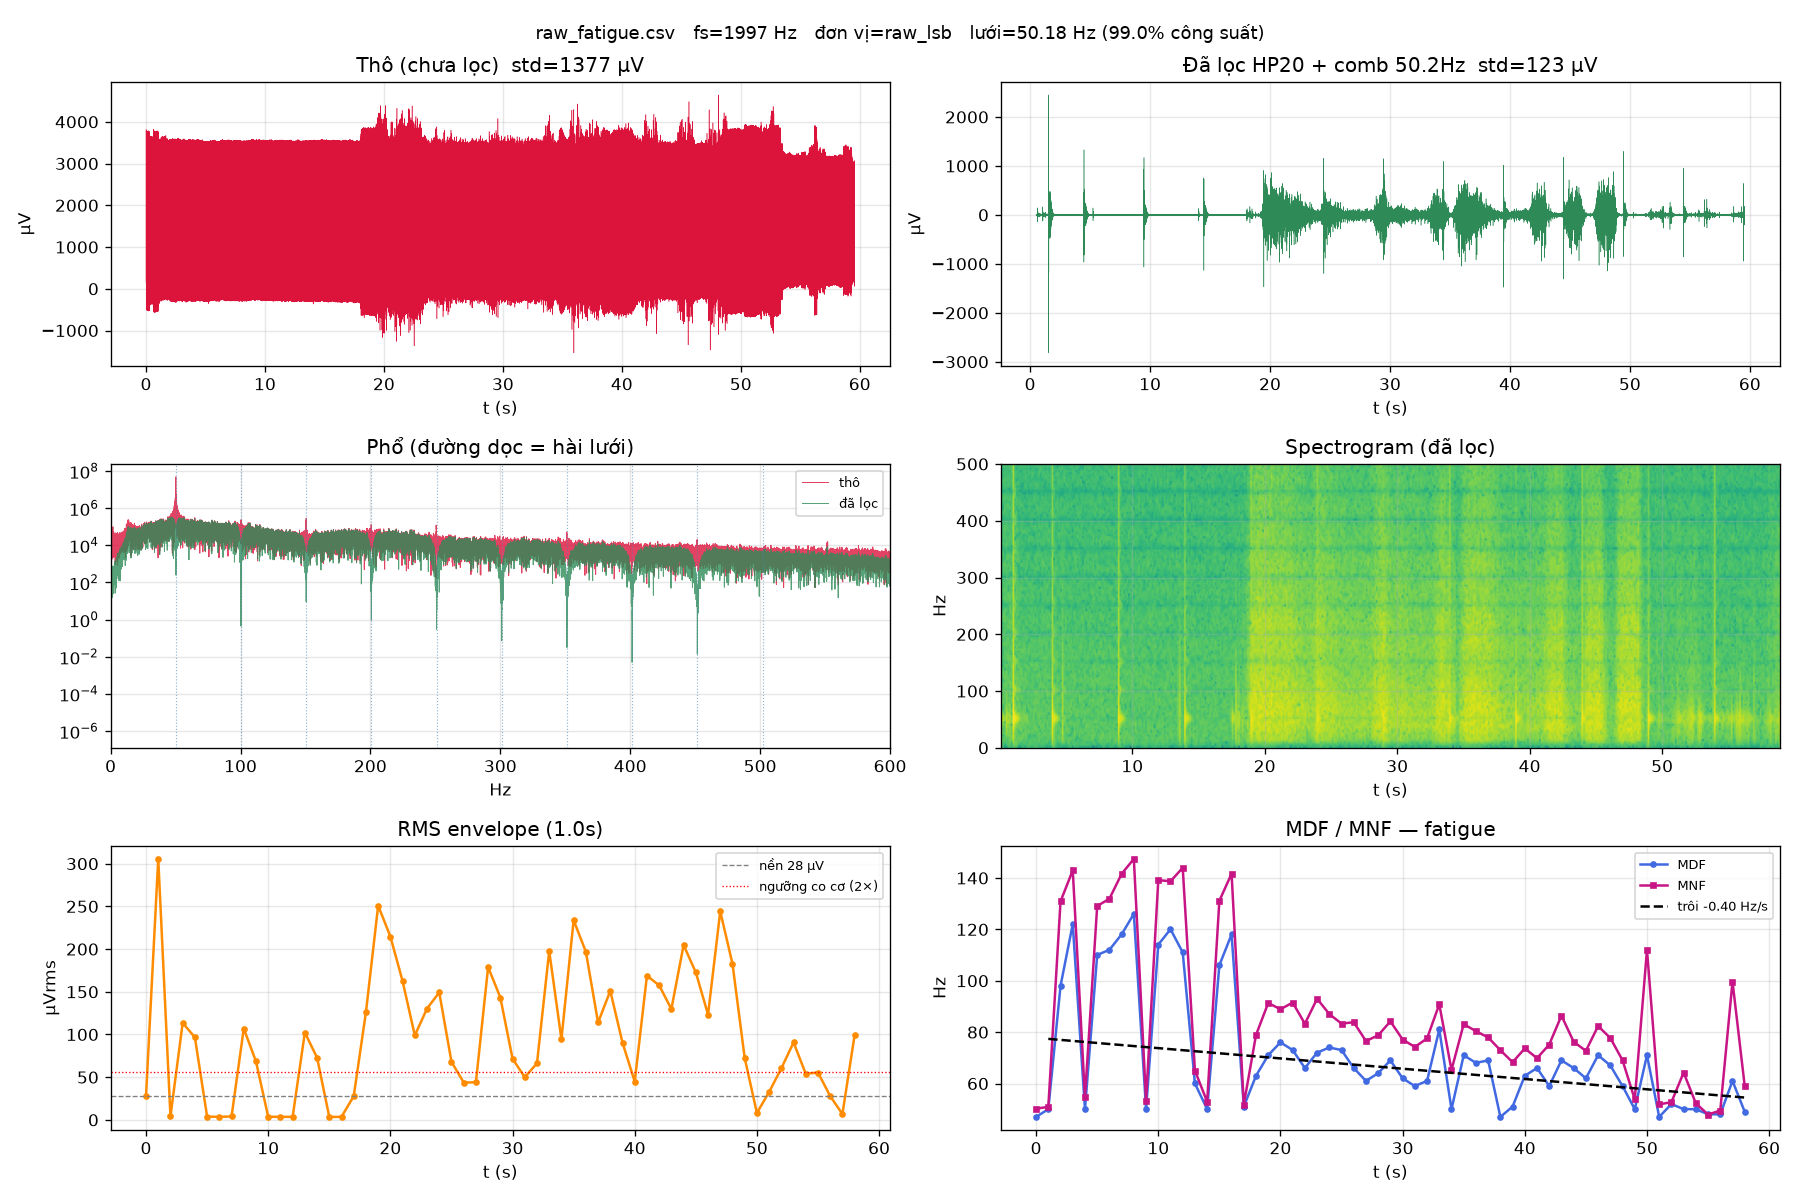
\includegraphics[width=0.98\textwidth]{figures/fig_pilot_raw_fatigue.png}
    \caption{Ví dụ ảnh phân tích log pilot 
    \texttt{raw\_fatigue.csv} của dự án. Đây là dữ liệu minh họa quy trình
    xử lý (dạng sóng, phổ, spectrogram, RMS, MDF/MNF), không phải kết quả
    xác nhận mỏi cơ; log và giới hạn diễn giải được truy về tài liệu và
    script trong kho firmware.}
    \label{fig:pilot-fatigue}
\end{figure}

% ============================================================
\section{Điều kiện để kết luận đáng tin}
\label{sec:conditions}

\subsection{Loại co cơ và điều kiện cơ học}
\label{sec:contraction-types}

Đặc trưng sEMG chỉ có ý nghĩa trong ngữ cảnh nhiệm vụ. Co đẳng trường giữ
ổn định tư thế và độ dài cơ, thường thuận lợi cho giả định gần dừng. Co
đồng tâm, lệch tâm và co động làm thay đổi hình học nguồn--điện cực, tăng
artifact và tạo phổ phi dừng; khi đó cần phân tích theo pha hoặc thời gian--
tần số \cite{mcmanus2020analysis,knaflitz1999time}.

\begin{table}[htbp]
\centering
\caption{Loại co cơ và hệ quả đối với phân tích sEMG}
\label{tab:contraction-types}
\begin{tabularx}{\textwidth}{@{}P{3.1cm}Y Y@{}}
\toprule
\textbf{Loại co} & \textbf{Đặc điểm cơ học} & \textbf{Hệ quả phân tích} \\
\midrule
Đẳng trường & Độ dài cơ và tư thế gần cố định, lực có thể giữ ở mức mục tiêu. & Thuận lợi hơn cho cửa sổ gần dừng và so sánh MNF/MDF. \\
Đồng tâm/lệch tâm & Cơ ngắn lại hoặc dài ra trong khi sinh lực. & Hình học nguồn--điện cực thay đổi; cần kiểm soát pha và nhiễu giả do chuyển động. \\
Co động & Có chuyển động khớp hoặc phối hợp nhiều cơ. & Cần phân tích thời gian--tần số, phân đoạn theo pha và có thể cần cảm biến chuyển động. \\
\bottomrule
\end{tabularx}
\end{table}

\subsection{Các nhãn tham chiếu: MVC, lực mục tiêu, task failure và RPE}
\label{sec:reference-labels}

Các nhãn tham chiếu đặt đặc trưng vào đúng ngữ cảnh. MVC là mức co tối đa
tự nguyện, thường dùng để chuẩn hóa biên độ; giá trị MVC phụ thuộc động
tác, tư thế, động lực và trạng thái người tham gia. Lực mục tiêu duy trì
được dùng trong thí nghiệm co đẳng trường; task failure là thời điểm không
còn duy trì được tiêu chí nhiệm vụ. RPE (rating of perceived exertion)
phản ánh cảm nhận gắng sức và không thay thế phép đo khả năng thực hiện
\cite{enoka2016translating}.

\subsection{Lặp lại và các biến cần báo cáo}
\label{sec:reporting}

Để kết quả có thể lặp lại, cần báo cáo tối thiểu các nhóm biến trong
Bảng~\ref{tab:reporting-checklist}. Danh sách này dựa trên các chuẩn báo
cáo EMG và CEDE-Check \cite{merletti1999standards,besomi2024cede,hermens2000development}.

\begin{table}[htbp]
\centering
\caption{Danh mục biến tối thiểu cần báo cáo cho một phép đo sEMG}
\label{tab:reporting-checklist}
\begin{tabularx}{\textwidth}{@{}P{3.4cm}Y@{}}
\toprule
\textbf{Nhóm biến} & \textbf{Nội dung cần ghi rõ} \\
\midrule
Đối tượng và nhiệm vụ & Cơ đo, bên cơ thể, tư thế, loại co, mức lực hoặc mô-men, tốc độ và thời lượng. \\
Điện cực & Loại, kích thước, vị trí, hướng, IED, điện cực tham chiếu và cách chuẩn bị da. \\
Chuỗi thu nhận & Gain, băng thông, loại lọc tương tự/số, chống alias, $f_s$, độ phân giải và kiểm tra clipping. \\
Phân tích & Độ dài cửa sổ, mức chồng lấp, hàm cửa sổ, phương pháp PSD và định nghĩa từng đặc trưng. \\
Chuẩn hóa và nhãn & MVC hoặc nhiệm vụ tham chiếu, tiêu chí onset/task failure, RPE nếu có và cách xử lý dữ liệu lỗi. \\
Thiết kế lặp lại & Số người, số lần lặp, số phiên, khoảng nghỉ và tiêu chí loại mẫu. \\
\bottomrule
\end{tabularx}
\end{table}

\subsection{Đo trực tiếp và suy luận: phạm vi kết luận của sEMG}
\label{sec:direct-vs-inference}

Bảng~\ref{tab:direct-vs-inference} tổng hợp các tầng kết luận. Nguyên tắc
cốt lõi là chỉ hiệu điện thế vi sai trên da là đại lượng đo trực tiếp; mọi
tầng phía trên đều cần điều kiện, thuật toán hoặc phép đo bổ sung
\cite{campanini2022fundamental,mcmanus2020analysis}.

\begin{table}[htbp]
\centering
\caption{Phân biệt đại lượng đo trực tiếp và suy luận từ sEMG bề mặt}
\label{tab:direct-vs-inference}
\begin{tabularx}{\textwidth}{@{}P{4.0cm}P{2.6cm}Y@{}}
\toprule
\textbf{Đối tượng} & \textbf{Loại} & \textbf{Điều kiện và ghi chú} \\
\midrule
Hiệu điện thế vi sai trên da & Đo trực tiếp & Đại lượng vật lý của phép đo; chịu ảnh hưởng giao diện, dẫn truyền thể tích và nhiễu. \\
ARV/MAV, RMS & Đại lượng dẫn xuất & Hàm xác định của tín hiệu trong cửa sổ; cần tín hiệu trung bình không và cửa sổ đủ dài. \\
PSD, MNF, MDF & Đại lượng dẫn xuất & Phụ thuộc cửa sổ, dải phân tích, $f_s$, cấu hình điện cực và phương pháp PSD. \\
Onset/offset & Suy luận có thuật toán & Phụ thuộc ngưỡng, cửa sổ và lọc; biểu diễn hoạt động điện của vùng thu. \\
Tuyển mộ và tần số từng MU & Suy luận & Cần kỹ thuật phân tách tín hiệu; một kênh thường không đủ. \\
Lực cơ, lực khớp & Suy luận & Quan hệ sEMG--lực phi tuyến và cục bộ; cần mô hình cùng dữ liệu hiệu chuẩn. \\
Chuyển động, vận tốc, tư thế & Suy luận & sEMG không đo trực tiếp chuyển động; nên có cảm biến bổ sung. \\
Mỏi cơ & Suy luận gián tiếp & MNF/MDF và biên độ là biểu hiện điện, không phải định nghĩa mỏi. \\
Hoạt động cơ lân cận & Suy luận & Có thể bị crosstalk che phủ; một kênh không tách được nguồn trong mọi điều kiện. \\
\bottomrule
\end{tabularx}
\end{table}

% ============================================================
\section{Tóm tắt chương}
\label{sec:ch2-summary}

Chương này đã trình bày chuỗi từ lệnh vận động đến tín hiệu sEMG trên da:
MU phát các điện thế hoạt động; SFAP của nhiều sợi tạo MUAP và MUAPT; dẫn
truyền thể tích làm suy giảm và làm trơn tín hiệu; cặp điện cực đo tổng
của nhiều nguồn cùng nhiễu. Tuyển mộ và mã hóa tần số phát xung làm thay đổi tổng
này, tạo nền tảng vật lý cho các đặc trưng biên độ và phổ.

Các hình trong chương giúp phân biệt nguồn tín hiệu, hình học đo và các
phép biến đổi xử lý; các bảng chỉ ra điều kiện cần để diễn giải. Ba kết
luận phương pháp luận là: sEMG đo hiệu điện thế vi sai trên da, qua đó
phản ánh tổng hợp hoạt động điện trong một vùng hữu hạn; ARV, RMS, MNF và
MDF là các đại lượng dẫn xuất phụ thuộc cấu hình; và mọi phát
biểu về lực, chuyển động hoặc mỏi đều là suy luận có điều kiện. Những
nguyên tắc này sẽ được dùng để đánh giá thông số phần cứng, firmware, dữ
liệu và kết quả thực nghiệm của hệ thống ở các phần tiếp theo.


% ==================== TÀI LIỆU THAM KHẢO ====================

\printbibliography[heading=bibintoc, title={Tài liệu tham khảo}]

\end{document}
